\documentclass[slidestop]{beamer}
\usepackage{graphicx}
\usepackage{amsmath}	% Advanced maths commands
\usepackage{amssymb}	% Extra maths symbols
\usepackage{datetime}
\usepackage{multirow}
\usepackage{epstopdf}
\usepackage{tikz}
\usepackage{xcolor}
\usepackage[normalem]{ulem}
\usepackage[outline]{contour}

\newdate{date}{21}{8}{2018}
\date{\displaydate{date}}

\usetikzlibrary{calc}
\usecolortheme{albatross}
\setbeamertemplate{background canvas} {% 

\begin{tikzpicture} 
    \shade [left color=blue!80!black,right color=blue!20!black] 
        (0,0) rectangle (\paperwidth,\paperheight); 
\end{tikzpicture} 
} 

\newcommand{\tkzpicmyps}[4]{\fill [fill=white](#1,#2) rectangle +(#3,#3*0.772727273) [path picture=
	{
		\node at (path picture bounding box.center) 
		{
			\includegraphics[height=#3cm,angle=-90]{#4}
		};
	}
];
}

\newcommand{\tkzpic}[5]{\fill [fill=white](#1,#2) rectangle +(#3,#4) [path picture=
	{
		\node at (path picture bounding box.center) 
		{
			\includegraphics[width=#3cm]{#5}
		};
	}
];
}
\newcommand{\tkzpich}[5]{\fill [fill=white](#1,#2) rectangle +(#3,#4) [path picture=
	{
		\node at (path picture bounding box.center) 
		{
			\includegraphics[height=#4cm]{#5}
		};
	}
];
}
\newcommand{\tkzpicwh}[5]{\fill [fill=white](#1,#2) rectangle +(#3,#4) [path picture=
	{
		\node at (path picture bounding box.center) 
		{
			\includegraphics[width=#3cm,height=#4cm]{#5}
		};
	}
];
}
\newcommand{\Msunp}{\;$\mathrm{M}_\odot$}
\newcommand{\Msun}{\;$\mathrm{M}_\odot$\;}
\newcommand{\Lsunp}{\;$\mathrm{L}_\odot$}
\newcommand{\Lsun}{\;$\mathrm{L}_\odot$\;}
\newcommand{\kms}{\;$\mathrm{km}\;\mathrm{s}^{-1}$\;}
\newcommand{\kmsp}{\;$\mathrm{km}\;\mathrm{s}^{-1}$}

%\usecolortheme[rgb={1.0,1.0,1.0}]{normal text}
\setbeamersize{text margin left=0.1cm,text margin right=0.1cm}
\tikzstyle{dashed}=                  [dash pattern=on 6pt off 6pt]
\usetikzlibrary{positioning}
\usetikzlibrary{decorations.pathmorphing}
\usetikzlibrary{decorations.pathreplacing}

\tikzset{snake it/.style={decorate, decoration=snake}}
%\usepackage{tikz-feynman}

\title{Exploding Stars, the Universe, and You}
\author{Dr. Brian W. Mulligan}
\institute{The University of Texas at Austin}

\begin{document}
\frame{
\maketitle
\begin{center} AoTATX \# 47 \end{center}
}

\frame{\frametitle{Pre-summary}
\begin{centering}
\vspace{0.5cm}
Supernova = Exploding star\hfill\\[14pt]
Factories for {\color{gray}neutron stars} \& {\color{black}\bf black holes}\\
{\scriptsize Only source of {\color{gray}neutron stars}}\\
{\scriptsize Maybe only source of {\color{black}\bf black holes}}\\[14pt]
Source of most elements${}^*$ heaver than oxygen in the Universe\\
{\scriptsize All of the {\color{red}iron} in your blood and {\color{yellow}calcium} in your bones were formed in supernovae}\\
{\scriptsize ${}^*$ elements heavier than {\color{green}copper} also come from {\color{gray}neutron star} mergers}\\
{\scriptsize ${}^*$ some elements heavier than {\color{magenta}strontium} also come from red giants}\\[14pt]
Thermonuclear supernovae reveal the presence of \color{magenta}{dark energy}.\\


\end{centering}
}

%\frame{\frametitle{Outline}\tableofcontents}

%\item Type Ia supernovae (SN~Ia)
%\item High velocity features in SN~Ia
%\item The compact circumstellar shell model \& interaction
%\item Synthetic spectra \& comparison to observations
%\end{itemize}
%}
%\setbeamertemplate{footline}{\insertsectionhead~\insertpagenumber / 10}

\frame{\frametitle{Three stars: a story : {\color{red} Just formed}}
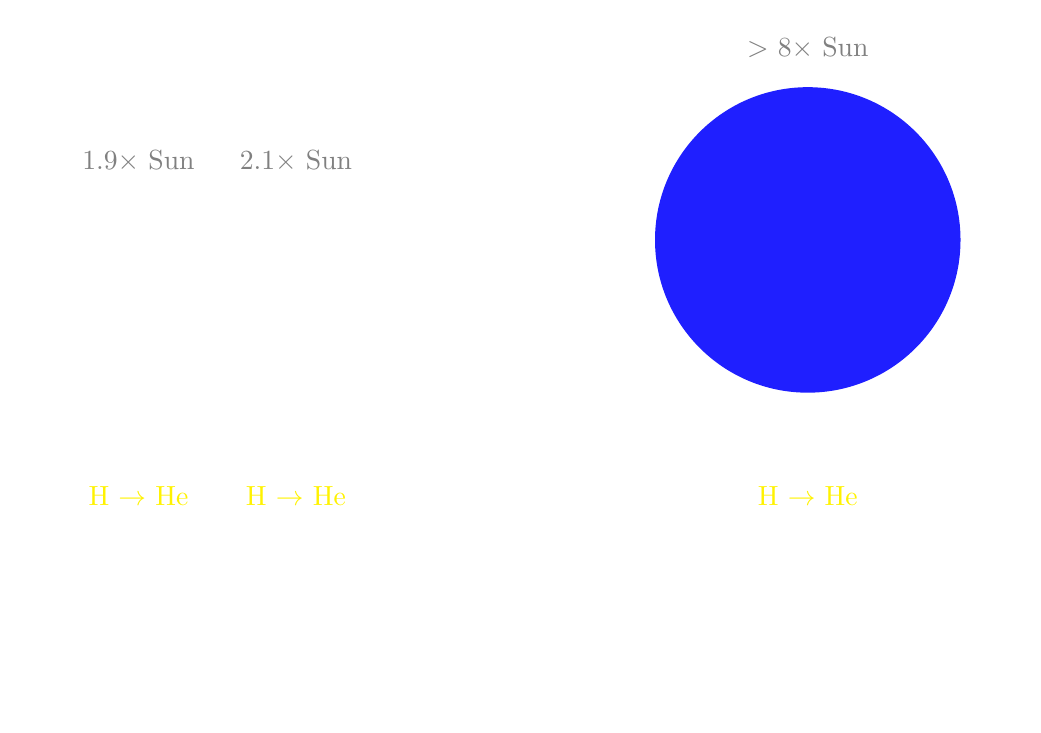
\begin{tikzpicture}
\draw[opacity=0] (0.1,0.1) rectangle (12.6,8.6);

\fill[white] (1.5,6) circle (0.5);
\fill[white] (3.5,6) circle (0.5);
\draw[white!50!black] (1.5,7) node {1.9$\times$ Sun};
\draw[white!50!black] (3.5,7) node {2.1$\times$ Sun};
\draw[yellow] (1.5,2.75) node {H $\rightarrow$ He};
\draw[yellow] (3.5,2.75) node {H $\rightarrow$ He};

\fill[white!12!blue] (10,6) circle (1.94);
\draw[white!50!black] (10,8.44) node {$>$ 8$\times$ Sun};
\draw[yellow] (10,2.75) node {H $\rightarrow$ He};
\end{tikzpicture}
}

\frame{\frametitle{An Open Cluster (NGC 6397)}
\begin{tikzpicture}
\draw[opacity=0] (0.1,0.1) rectangle (12.6,8.6);

\tkzpic{0.9}{0.75}{11}{8.25}{Pictures/hubbleimage1stscihp1824am2000x1500};
\draw[yellow] (6.4,0.85) node[font=\tiny] {Credits: NASA, ESA, and T. Brown and S. Casertano (STScI); Acknowledgement: NASA, ESA, and J. Anderson (STScI)};
\end{tikzpicture}
}

\frame{\frametitle{Three stars: a story : {\color{red} 1 Million Years Old}}
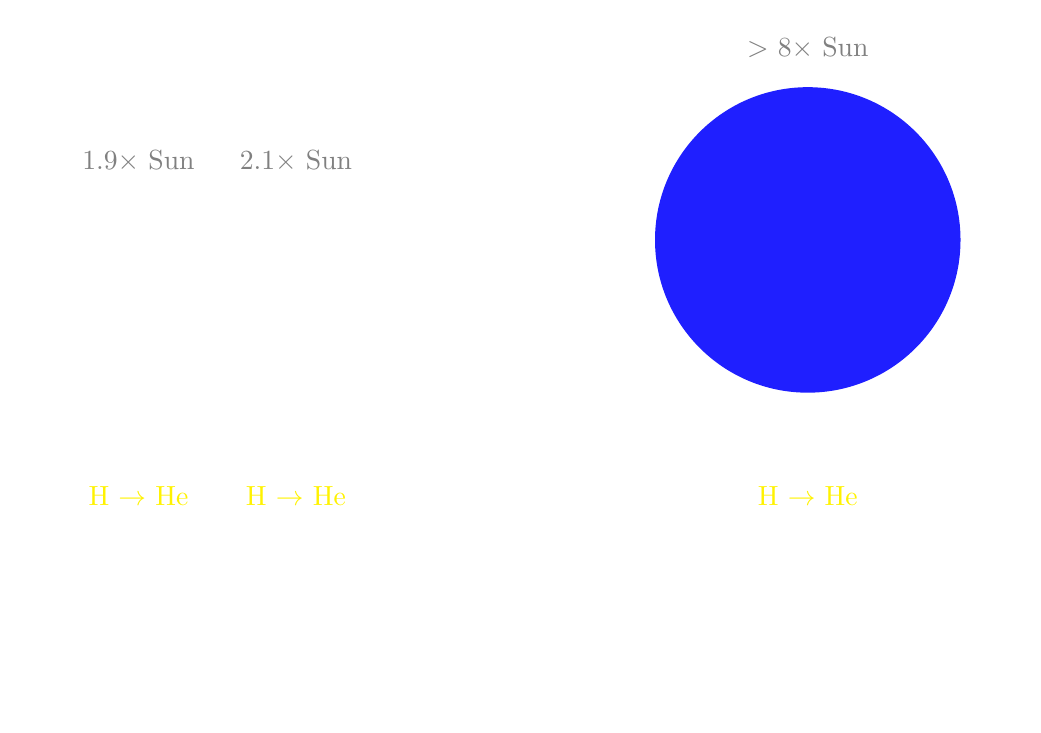
\begin{tikzpicture}
\draw[opacity=0] (0.1,0.1) rectangle (12.6,8.6);


\fill[white] (1.5,6) circle (0.5);
\fill[white] (3.5,6) circle (0.5);
\draw[white!50!black] (1.5,7) node {1.9$\times$ Sun};
\draw[white!50!black] (3.5,7) node {2.1$\times$ Sun};
\draw[yellow] (1.5,2.75) node {H $\rightarrow$ He};
\draw[yellow] (3.5,2.75) node {H $\rightarrow$ He};


\fill[white!12!blue] (10,6) circle (1.94);
\draw[white!50!black] (10,8.44) node {$>$ 8$\times$ Sun};
\draw[yellow] (10,2.75) node {H $\rightarrow$ He};
\end{tikzpicture}
}

\frame{\frametitle{Three stars: a story : {\color{red} 2 Million Years Old}}
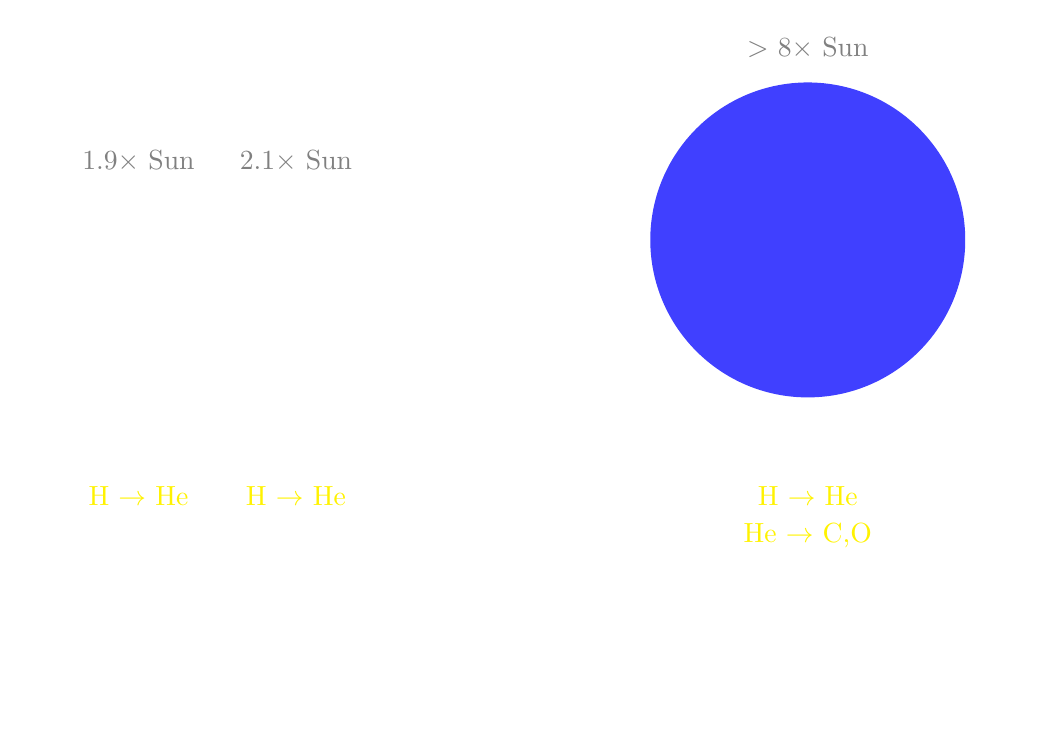
\begin{tikzpicture}
\draw[opacity=0] (0.1,0.1) rectangle (12.6,8.6);


\fill[white] (1.5,6) circle (0.5);
\fill[white] (3.5,6) circle (0.5);
\draw[white!50!black] (1.5,7) node {1.9$\times$ Sun};
\draw[white!50!black] (3.5,7) node {2.1$\times$ Sun};
\draw[yellow] (1.5,2.75) node {H $\rightarrow$ He};
\draw[yellow] (3.5,2.75) node {H $\rightarrow$ He};


\fill[white!25!blue] (10,6) circle (2.0);
\draw[white!50!black] (10,8.44) node {$>$ 8$\times$ Sun};
\draw[yellow] (10,2.75) node {H $\rightarrow$ He};
\draw[yellow] (10,2.25) node {He $\rightarrow$ C,O};
\end{tikzpicture}
}

\frame{\frametitle{Three stars: a story : {\color{red} 3 Million Years Old}}
\begin{tikzpicture}
\draw[opacity=0] (0.1,0.1) rectangle (12.6,8.6);


\draw[white!50!black] (1.5,7) node {1.9$\times$ Sun};
\draw[white!50!black] (3.5,7) node {2.1$\times$ Sun};
\fill[white] (1.5,6) circle (0.5);
\fill[white] (3.5,6) circle (0.5);
\draw[yellow] (1.5,2.75) node {H $\rightarrow$ He};
\draw[yellow] (3.5,2.75) node {H $\rightarrow$ He};

\fill[black] (10,6) circle (0.000011905);

\end{tikzpicture}
}

\frame{\frametitle{Three stars: a story : {\color{red} 2 Million Years Old}}
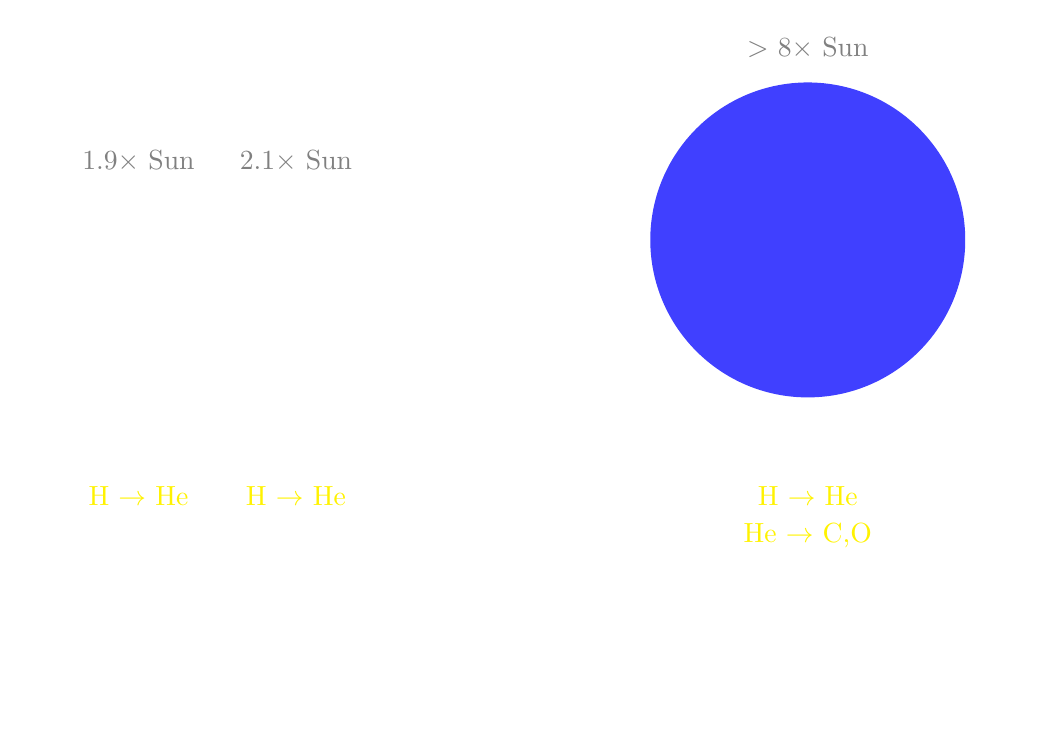
\begin{tikzpicture}
\draw[opacity=0] (0.1,0.1) rectangle (12.6,8.6);


\fill[white] (1.5,6) circle (0.5);
\fill[white] (3.5,6) circle (0.5);
\draw[white!50!black] (1.5,7) node {1.9$\times$ Sun};
\draw[white!50!black] (3.5,7) node {2.1$\times$ Sun};
\draw[yellow] (1.5,2.75) node {H $\rightarrow$ He};
\draw[yellow] (3.5,2.75) node {H $\rightarrow$ He};

\fill[white!25!blue] (10,6) circle (2.0);
\draw[white!50!black] (10,8.44) node {$>$ 8$\times$ Sun};
\draw[yellow] (10,2.75) node {H $\rightarrow$ He};
\draw[yellow] (10,2.25) node {He $\rightarrow$ C,O};
\end{tikzpicture}
}

\frame{\frametitle{Three stars: a story : {\color{red} 2.5 Million Years Old}}
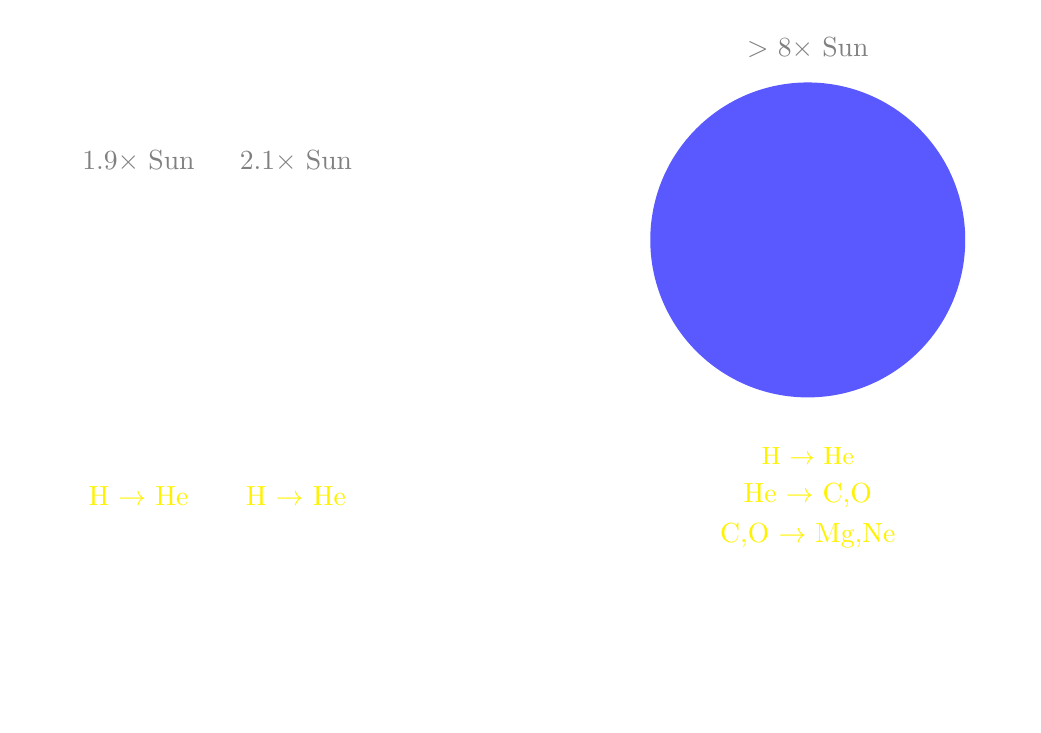
\begin{tikzpicture}
\draw[opacity=0] (0.1,0.1) rectangle (12.6,8.6);


\fill[white] (1.5,6) circle (0.5);
\fill[white] (3.5,6) circle (0.5);
\draw[white!50!black] (1.5,7) node {1.9$\times$ Sun};
\draw[white!50!black] (3.5,7) node {2.1$\times$ Sun};
\draw[yellow] (1.5,2.75) node {H $\rightarrow$ He};
\draw[yellow] (3.5,2.75) node {H $\rightarrow$ He};

\draw[white!50!black] (10,8.44) node {$>$ 8$\times$ Sun};
\draw[yellow] (10,3.25) node {\small H $\rightarrow$ He};
\draw[yellow] (10,2.75) node {He $\rightarrow$ C,O};
\draw[yellow] (10,2.25) node {C,O $\rightarrow$ Mg,Ne};
\fill[white!35!blue] (10,6) circle (2.0);
\end{tikzpicture}
}

\frame{\frametitle{Three stars: a story : {\color{red} 2.55 Million Years Old}}
\begin{tikzpicture}
\draw[opacity=0] (0.1,0.1) rectangle (12.6,8.6);


\fill[white] (1.5,6) circle (0.5);
\fill[white] (3.5,6) circle (0.5);
\draw[white!50!black] (1.5,7) node {1.9$\times$ Sun};
\draw[white!50!black] (3.5,7) node {2.1$\times$ Sun};
\draw[yellow] (1.5,2.75) node {H $\rightarrow$ He};
\draw[yellow] (3.5,2.75) node {H $\rightarrow$ He};

\fill[white] (10,6) circle (2.5);
\draw[white!50!black] (10,8.44) node {$>$ 8$\times$ Sun};
\draw[yellow] (10,3.75) node {H $\rightarrow$ He};
\draw[yellow] (10,3.25) node {He $\rightarrow$ C,O};
\draw[yellow] (10,2.75) node {C,O $\rightarrow$ Mg,Ne};
\draw[yellow] (10,2.25) node {Mg,Ne $\rightarrow$ Si,S,Ca};
\end{tikzpicture}
}

\frame{\frametitle{Three stars: a story : {\color{red} 2.56 Million Years Old}}
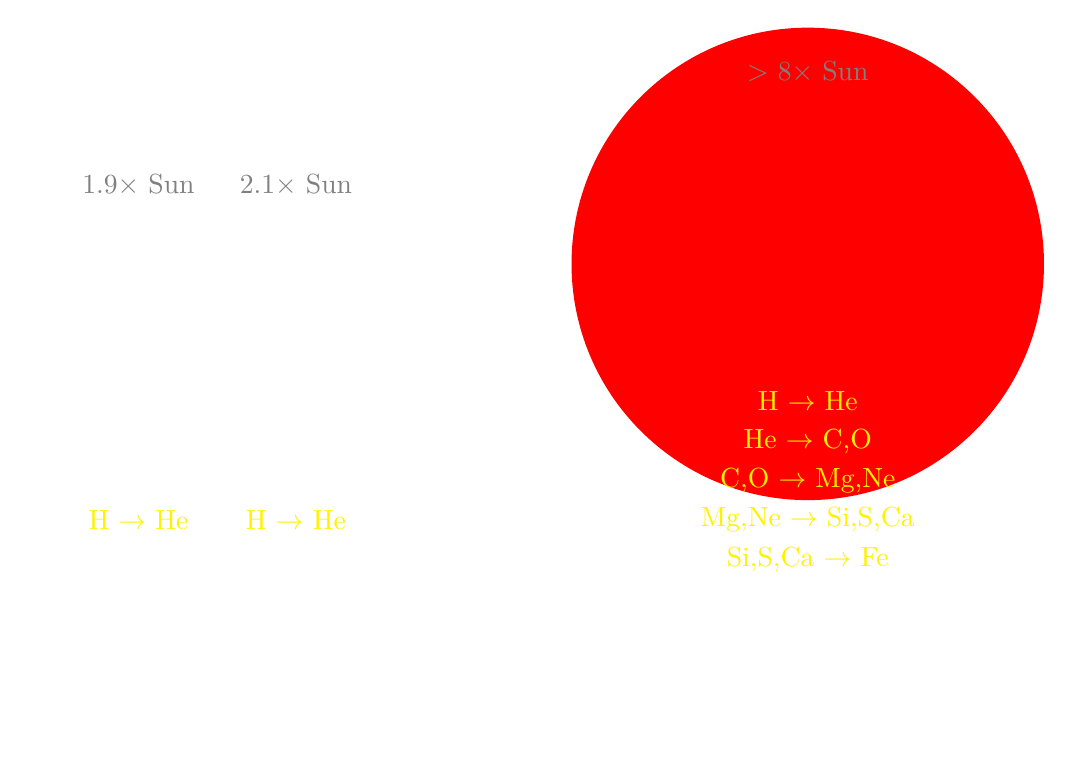
\begin{tikzpicture}
\draw[opacity=0] (0.1,0.1) rectangle (12.6,8.6);


\draw[white!50!black] (1.5,7) node {1.9$\times$ Sun};
\draw[white!50!black] (3.5,7) node {2.1$\times$ Sun};
\fill[white] (1.5,6) circle (0.5);
\fill[white] (3.5,6) circle (0.5);
\draw[yellow] (1.5,2.75) node {H $\rightarrow$ He};
\draw[yellow] (3.5,2.75) node {H $\rightarrow$ He};

\fill[red] (10,6) circle (3.0);
\draw[white!50!black] (10,8.44) node {$>$ 8$\times$ Sun};
\draw[yellow] (10,4.25) node {H $\rightarrow$ He};
\draw[yellow] (10,3.75) node {He $\rightarrow$ C,O};
\draw[yellow] (10,3.25) node {C,O $\rightarrow$ Mg,Ne};
\draw[yellow] (10,2.75) node {Mg,Ne $\rightarrow$ Si,S,Ca};
\draw[yellow] (10,2.25) node {Si,S,Ca $\rightarrow$ Fe};
\end{tikzpicture}
}

\frame{\frametitle{Three stars: a story : {\color{red} 2.561 Million Years Old}}
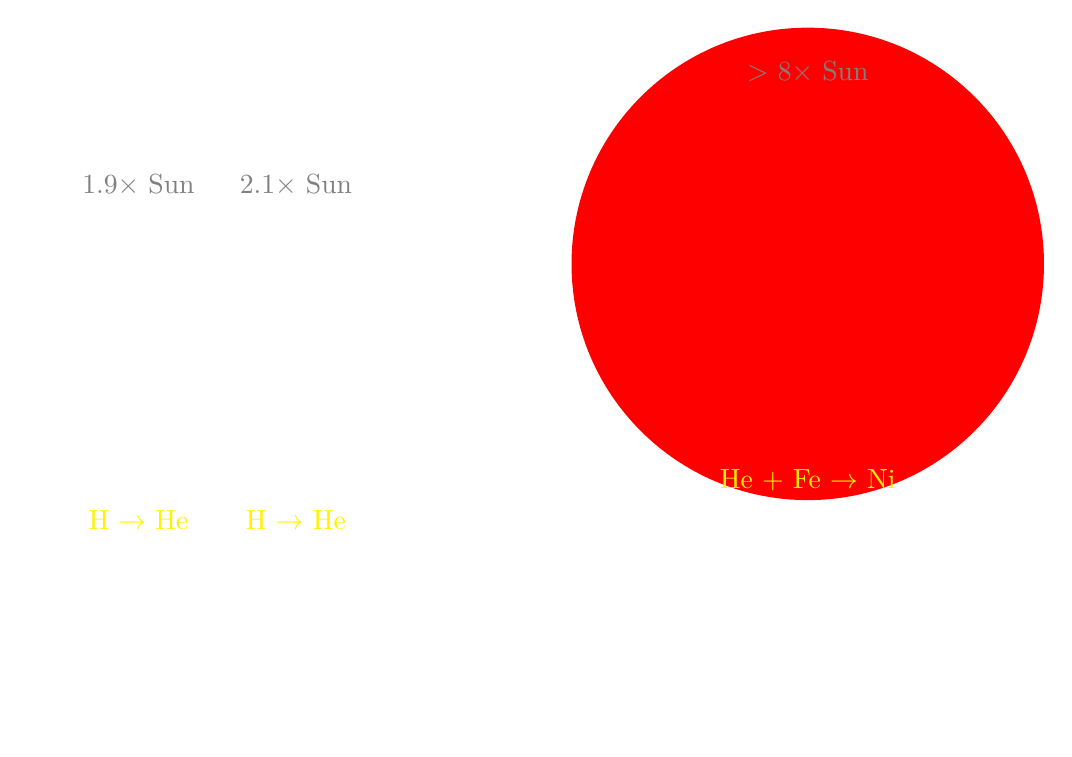
\begin{tikzpicture}
\draw[opacity=0] (0.1,0.1) rectangle (12.6,8.6);


\fill[white] (1.5,6) circle (0.5);
\fill[white] (3.5,6) circle (0.5);
\draw[white!50!black] (1.5,7) node {1.9$\times$ Sun};
\draw[white!50!black] (3.5,7) node {2.1$\times$ Sun};
\draw[yellow] (1.5,2.75) node {H $\rightarrow$ He};
\draw[yellow] (3.5,2.75) node {H $\rightarrow$ He};

\fill[red] (10,6) circle (3.0);
\draw[white!50!black] (10,8.44) node {$>$ 8$\times$ Sun};
\draw[yellow] (10,3.25) node {He + Fe $\rightarrow$ Ni};
\end{tikzpicture}
}

\frame{\frametitle{Three stars: a story : {\color{red} 2.561 Million Years Old}}
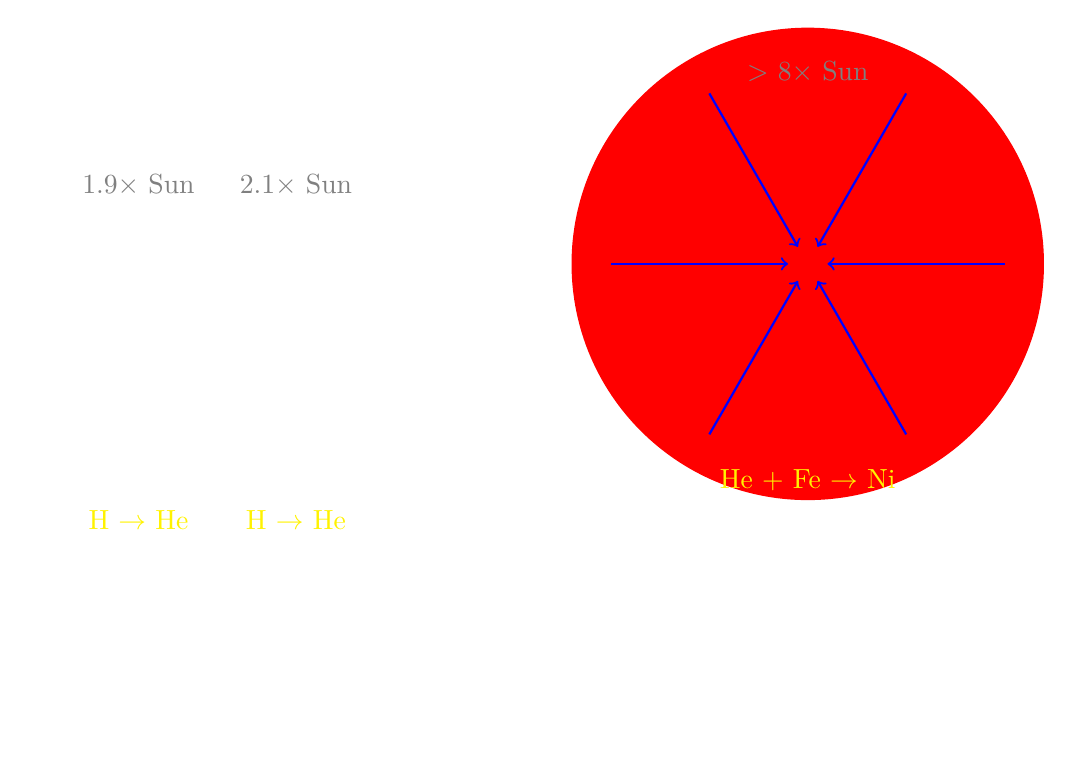
\begin{tikzpicture}
\draw[opacity=0] (0.1,0.1) rectangle (12.6,8.6);


\fill[white] (1.5,6) circle (0.5);
\fill[white] (3.5,6) circle (0.5);
\draw[white!50!black] (1.5,7) node {1.9$\times$ Sun};
\draw[white!50!black] (3.5,7) node {2.1$\times$ Sun};
\draw[yellow] (1.5,2.75) node {H $\rightarrow$ He};
\draw[yellow] (3.5,2.75) node {H $\rightarrow$ He};

\fill[red] (10,6) circle (3.0);
\draw[white!50!black] (10,8.44) node {$>$ 8$\times$ Sun};
\foreach \x in {0,60,-60,120,-120,180}
{
	\draw[blue,thick,->] (10,6)++(\x:2.5) -- +(\x:-2.25);
} 
\draw[yellow] (10,3.25) node {He + Fe $\rightarrow$ Ni};
\end{tikzpicture}
}

\frame{\frametitle{Three stars: a story : {\color{red} 2.561 Million Years Old + 1 second}}
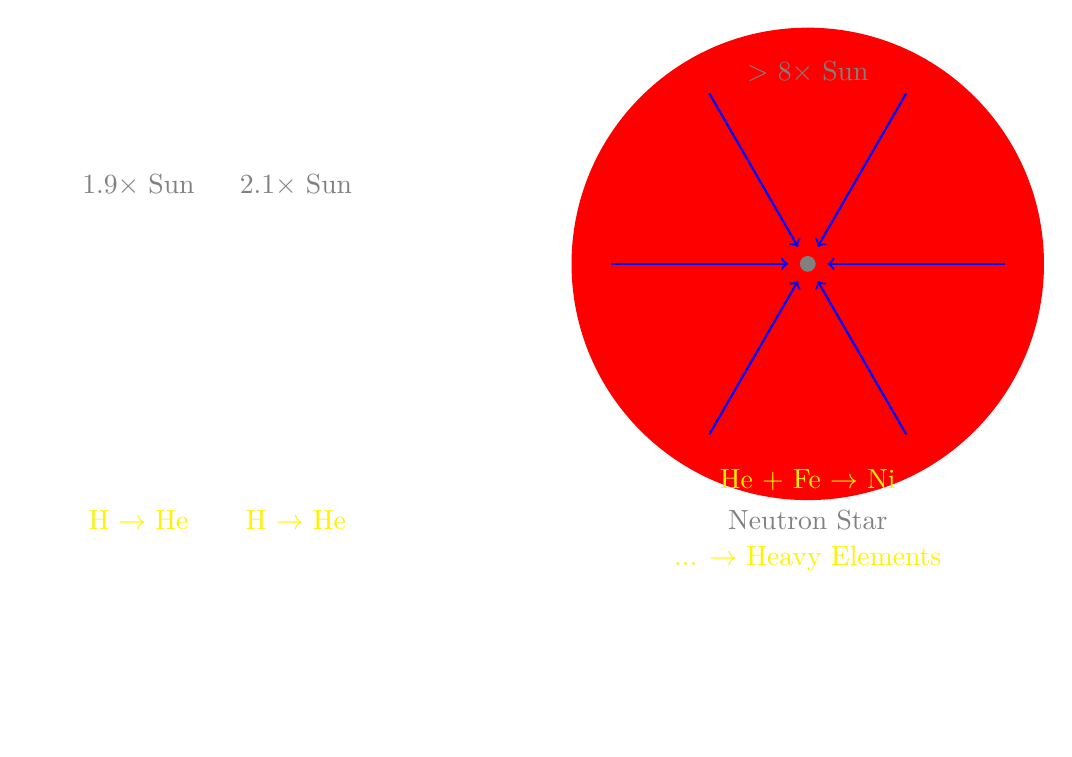
\begin{tikzpicture}
\draw[opacity=0] (0.1,0.1) rectangle (12.6,8.6);


\fill[white] (1.5,6) circle (0.5);
\fill[white] (3.5,6) circle (0.5);
\draw[white!50!black] (1.5,7) node {1.9$\times$ Sun};
\draw[white!50!black] (3.5,7) node {2.1$\times$ Sun};
\draw[yellow] (1.5,2.75) node {H $\rightarrow$ He};
\draw[yellow] (3.5,2.75) node {H $\rightarrow$ He};

\fill[red] (10,6) circle (3.0);
\draw[white!50!black] (10,8.44) node {$>$ 8$\times$ Sun};
\fill[gray] (10,6) circle (0.1);
\foreach \x in {0,60,-60,120,-120,180}
{
	\draw[blue,thick,->] (10,6)++(\x:2.5) -- +(\x:-2.25);
} 
\draw[yellow] (10,3.25) node {He + Fe $\rightarrow$ Ni};
\draw[gray] (10,2.75) node {Neutron Star};
\draw[yellow] (10,2.25) node {... $\rightarrow$ Heavy Elements};
\end{tikzpicture}
}


\frame{\frametitle{Three stars: a story : {\color{red} 2.561 Million Years Old + 1.001 sec.}}
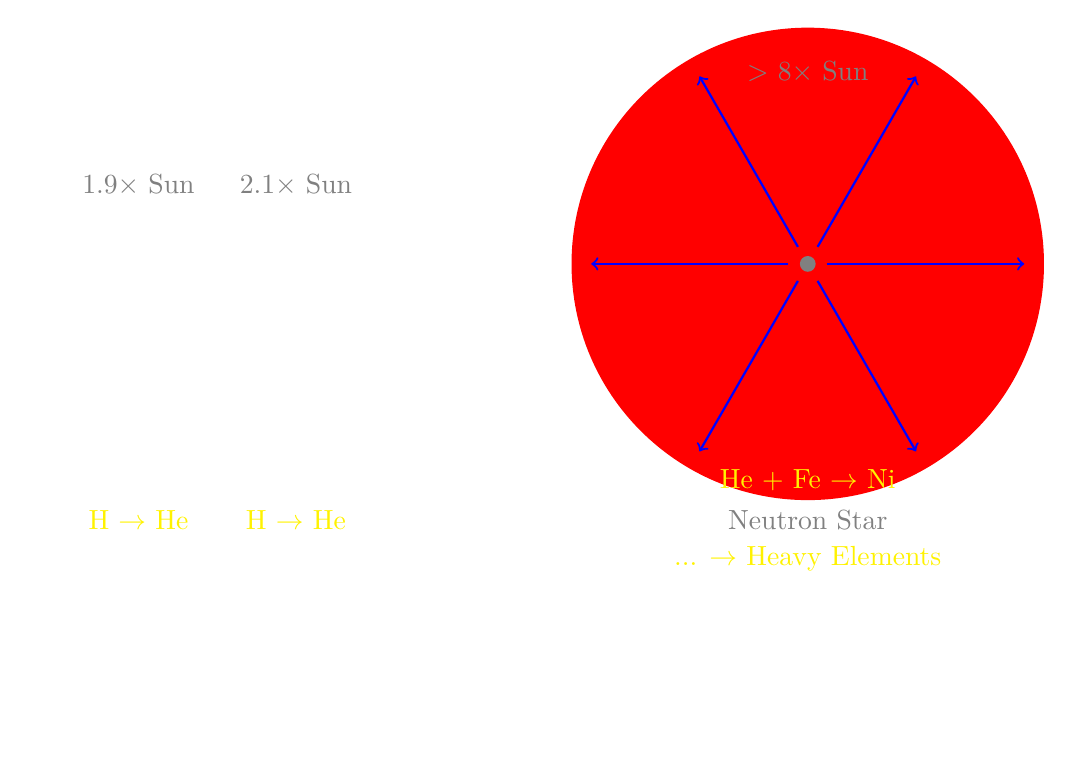
\begin{tikzpicture}
\draw[opacity=0] (0.1,0.1) rectangle (12.6,8.6);


\fill[white] (1.5,6) circle (0.5);
\fill[white] (3.5,6) circle (0.5);
\draw[white!50!black] (1.5,7) node {1.9$\times$ Sun};
\draw[white!50!black] (3.5,7) node {2.1$\times$ Sun};
\draw[yellow] (1.5,2.75) node {H $\rightarrow$ He};
\draw[yellow] (3.5,2.75) node {H $\rightarrow$ He};

\fill[red] (10,6) circle (3.0);
\draw[white!50!black] (10,8.44) node {$>$ 8$\times$ Sun};
\fill[gray] (10,6) circle (0.1);
\foreach \x in {0,60,-60,120,-120,180}
{
	\draw[blue,thick,->] (10,6)++(\x:0.25) -- +(\x:2.5);
} 
\draw[yellow] (10,3.25) node {He + Fe $\rightarrow$ Ni};
\draw[gray] (10,2.75) node {Neutron Star};
\draw[yellow] (10,2.25) node {... $\rightarrow$ Heavy Elements};
\end{tikzpicture}
}

\frame{\frametitle{Three stars: a story : {\color{red} 2.561 Million Years Old + 1.0011 sec.}}
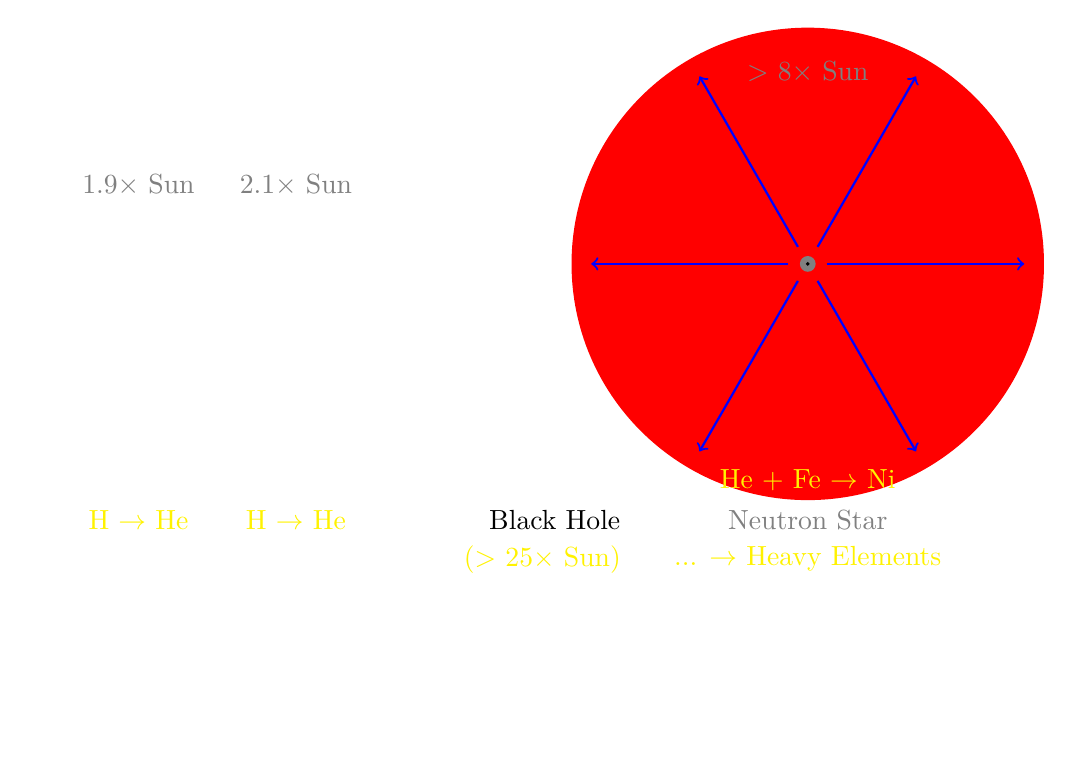
\begin{tikzpicture}
\draw[opacity=0] (0.1,0.1) rectangle (12.6,8.6);


\fill[white] (1.5,6) circle (0.5);
\fill[white] (3.5,6) circle (0.5);
\draw[white!50!black] (1.5,7) node {1.9$\times$ Sun};
\draw[white!50!black] (3.5,7) node {2.1$\times$ Sun};
\draw[yellow] (1.5,2.75) node {H $\rightarrow$ He};
\draw[yellow] (3.5,2.75) node {H $\rightarrow$ He};

\fill[red] (10,6) circle (3.0);
\foreach \x in {0,60,-60,120,-120,180}
{
	\draw[blue,thick,->] (10,6)++(\x:0.25) -- +(\x:2.5);
} 
\draw[white!50!black] (10,8.44) node {$>$ 8$\times$ Sun};
\fill[gray] (10,6) circle (0.1);
\fill[black] (10,6) circle (0.025);
\draw[yellow] (10,3.25) node {He + Fe $\rightarrow$ Ni};
\draw[gray] (10,2.75) node {Neutron Star};
\draw[yellow] (10,2.25) node {... $\rightarrow$ Heavy Elements};
\draw[black,thick] (7.75,2.75) node[left] {Black Hole};
\draw[yellow] (7.75,2.25) node[left] {($>$ 25$\times$ Sun)};
\end{tikzpicture}
}

\frame{\frametitle{A supernova remnant: the Crab Neblua\\ {\small \color{red} about 1000 years after the explosion}}
\begin{tikzpicture}
\draw[opacity=0] (0.1,0.1) rectangle (12.6,8.6);

\tkzpic{0.9}{0.2}{11}{8.25}{Pictures/STSCI-H-p1721a-m-2000x2000};
\draw[yellow] (6.4,1.10) node[font=\tiny] {Credit: NASA, ESA, G. Dubner (IAFE, CONICET-University of Buenos Aires) et al.; A. Loll et al.; T. Temim et al.;}; 
\draw[yellow] (6.4,0.85) node[font=\tiny] {F. Seward et al.; VLA/NRAO/AUI/NSF; Chandra/CXC; Spitzer/JPL-Caltech; XMM-Newton/ESA; and Hubble/STScI};
\end{tikzpicture}
}

\frame{\frametitle{A supernova remnant: the Crab Neblua\\ {\small \color{red} about 1000 years after the explosion}}
\begin{tikzpicture}
\draw[opacity=0] (0.1,0.1) rectangle (12.6,8.6);

\tkzpic{0.9}{0.2}{11}{8.25}{Pictures/STSCI-H-p1721a-m-2000x2000};
\draw[yellow] (2.5,7.95) -- (2.5,8.0) -- (10.3,8.0) -- (10.3,7.95);
\draw[yellow] (6.4,8.25) node {11 light years};
\draw[yellow!50!red] (6.4,4.325) -- (11.0,5) node[right] {Neutron};
\draw[yellow!50!red] (11.0,4.5) node[right] {Star};
\draw[yellow!50!red] (6.4,4.95) -- (11.0,5.625) node[right] {Hot gas};
\draw[yellow!50!red] (6.4,6.95) -- (11.0,7.625) node[right] {Dust};

\draw[yellow] (6.4,1.10) node[font=\tiny] {Credit: NASA, ESA, G. Dubner (IAFE, CONICET-University of Buenos Aires) et al.; A. Loll et al.; T. Temim et al.;}; 
\draw[yellow] (6.4,0.85) node[font=\tiny] {F. Seward et al.; VLA/NRAO/AUI/NSF; Chandra/CXC; Spitzer/JPL-Caltech; XMM-Newton/ESA; and Hubble/STScI};
\end{tikzpicture}
}

\frame{\frametitle{A supernova remnant: the Veil Neblua\\ {\small \color{red} about 10000 years after the explosion}}
\begin{tikzpicture}
\draw[opacity=0] (0.1,0.1) rectangle (12.6,8.6);

\tkzpic{0.9}{0.2}{11}{8.25}{Pictures/heic0712d-wallpaper};
\draw[yellow] (2.5,7.95) -- (2.5,8.0) -- (10.3,8.0) -- (10.3,7.95);
\draw[yellow] (6.4,8.25) node {50 light years};
\draw[yellow!50!red] (8.4,6.95) -- (11.0,7.075) node[right] {Dust};
\draw[yellow] (6.4,1.10) node[font=\tiny] {Credit: NASA, ESA, the Hubble Heritage (STScI/AURA)-ESA/Hubble Collaboration, and the Digitized Sky Survey 2}; 
\draw[yellow] (6.4,0.85) node[font=\tiny] {Acknowledgment: J. Hester (Arizona State University) and Davide De Martin (ESA/Hubble)};
\end{tikzpicture}
}

\frame{\frametitle{Three stars: a story : {\color{red} 3 Million Years Old}}
\begin{tikzpicture}
\draw[opacity=0] (0.1,0.1) rectangle (12.6,8.6);


\fill[white] (1.5,6) circle (0.5);
\fill[white] (3.5,6) circle (0.5);
\draw[white!50!black] (1.5,7) node {1.9$\times$ Sun};
\draw[white!50!black] (3.5,7) node {2.1$\times$ Sun};
\draw[yellow] (1.5,2.75) node {H $\rightarrow$ He};
\draw[yellow] (3.5,2.75) node {H $\rightarrow$ He};

\draw[white!50!black] (10,8.44) node {10$\times$ Sun Black Hole};
\fill[black] (10,6) circle (0.05);

\end{tikzpicture}
}
\frame{\frametitle{Three stars: a story : {\color{red} 5 Million Years Old}}
\begin{tikzpicture}
\draw[opacity=0] (0.1,0.1) rectangle (12.6,8.6);


\fill[white] (1.5,6) circle (0.5);
\fill[white] (3.5,6) circle (0.5);
\draw[white!50!black] (1.5,7) node {1.9$\times$ Sun};
\draw[white!50!black] (3.5,7) node {2.1$\times$ Sun};
\draw[yellow] (1.5,2.75) node {H $\rightarrow$ He};
\draw[yellow] (3.5,2.75) node {H $\rightarrow$ He};

\draw[white!50!black] (10,8.44) node {10$\times$ Sun Black Hole};
\fill[black] (10,6) circle (0.05);

\end{tikzpicture}
}

\frame{\frametitle{Three stars: a story : {\color{red} 50 Million Years Old}}
\begin{tikzpicture}
\draw[opacity=0] (0.1,0.1) rectangle (12.6,8.6);


\fill[white] (1.5,6) circle (0.5);
\fill[white] (3.5,6) circle (0.5);
\draw[white!50!black] (1.5,7) node {1.9$\times$ Sun};
\draw[white!50!black] (3.5,7) node {2.1$\times$ Sun};
\draw[yellow] (1.5,2.75) node {H $\rightarrow$ He};
\draw[yellow] (3.5,2.75) node {H $\rightarrow$ He};

\draw[white!50!black] (10,8.44) node {10$\times$ Sun Black Hole};
\fill[black] (10,6) circle (0.05);

\end{tikzpicture}
}

\frame{\frametitle{Three stars: a story : {\color{red} 100 Million Years Old}}
\begin{tikzpicture}
\draw[opacity=0] (0.1,0.1) rectangle (12.6,8.6);


\fill[white] (1.5,6) circle (0.5);
\fill[white] (3.5,6) circle (0.5);
\draw[white!50!black] (1.5,7) node {1.9$\times$ Sun};
\draw[white!50!black] (3.5,7) node {2.1$\times$ Sun};
\draw[yellow] (1.5,2.75) node {H $\rightarrow$ He};
\draw[yellow] (3.5,2.75) node {H $\rightarrow$ He};

\draw[white!50!black] (10,8.44) node {10$\times$ Sun Black Hole};
\fill[black] (10,6) circle (0.05);

\end{tikzpicture}
}

\frame{\frametitle{Three stars: a story : {\color{red} 500 Million Years Old}}
\begin{tikzpicture}
\draw[opacity=0] (0.1,0.1) rectangle (12.6,8.6);


\fill[white] (1.5,6) circle (0.5);
\fill[white] (3.5,6) circle (0.5);
\draw[white!50!black] (1.5,7) node {1.9$\times$ Sun};
\draw[white!50!black] (3.5,7) node {2.1$\times$ Sun};
\draw[yellow] (1.5,2.75) node {H $\rightarrow$ He};
\draw[yellow] (3.5,2.75) node {H $\rightarrow$ He};

\draw[white!50!black] (10,8.44) node {10$\times$ Sun Black Hole};
\fill[black] (10,6) circle (0.05);

\end{tikzpicture}
}

\frame{\frametitle{Three stars: a story : {\color{red} 1 Billion Years Old}}
\begin{tikzpicture}
\draw[opacity=0] (0.1,0.1) rectangle (12.6,8.6);


\fill[white] (1.5,6) circle (0.5);
\fill[white] (3.5,6) circle (0.5);
\draw[white!50!black] (1.5,7) node {1.9$\times$ Sun};
\draw[white!50!black] (3.5,7) node {2.1$\times$ Sun};
\draw[yellow] (1.5,2.75) node {H $\rightarrow$ He};
\draw[yellow] (3.5,2.75) node {H $\rightarrow$ He};

\draw[white!50!black] (10,8.44) node {10$\times$ Sun Black Hole};
\fill[black] (10,6) circle (0.05);

\end{tikzpicture}
}

\frame{\frametitle{Three stars: a story : {\color{red} 1.5 Billion Years Old}}
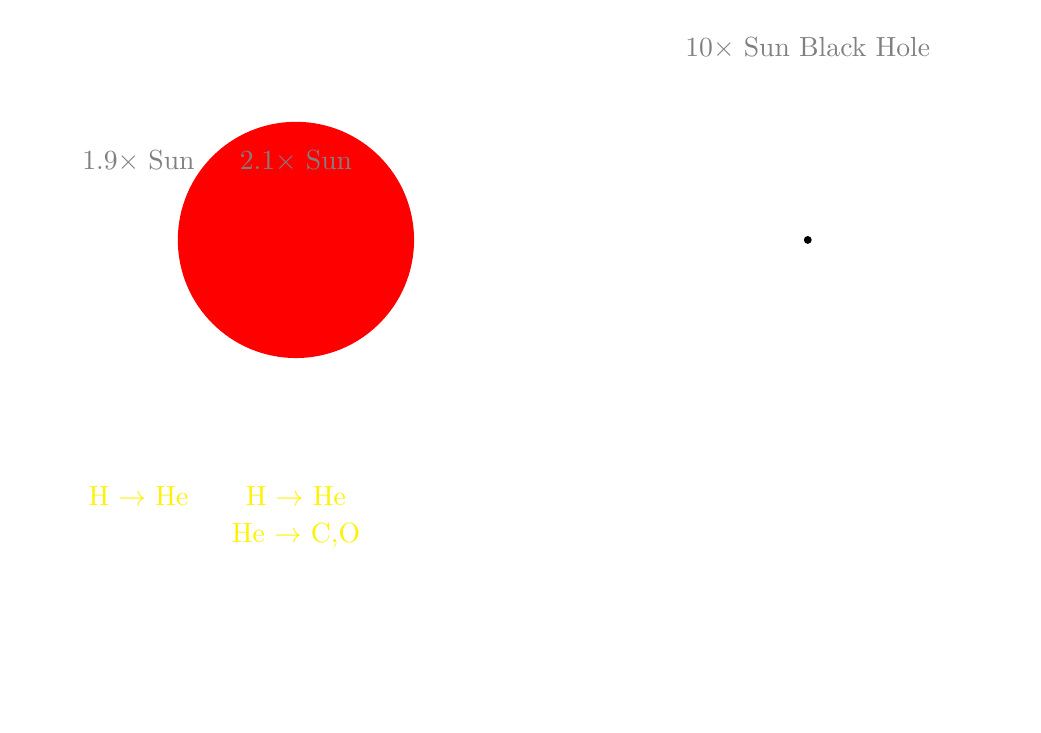
\begin{tikzpicture}
\draw[opacity=0] (0.1,0.1) rectangle (12.6,8.6);


\fill[white] (1.5,6) circle (0.5);
\fill[red] (3.5,6) circle (1.5);
\draw[white!50!black] (1.5,7) node {1.9$\times$ Sun};
\draw[white!50!black] (3.5,7) node {2.1$\times$ Sun};
\draw[yellow] (1.5,2.75) node {H $\rightarrow$ He};
\draw[yellow] (3.5,2.75) node {H $\rightarrow$ He};
\draw[yellow] (3.5,2.25) node {He $\rightarrow$ C,O};

\draw[white!50!black] (10,8.44) node {10$\times$ Sun Black Hole};
\fill[black] (10,6) circle (0.05);

\end{tikzpicture}
}

\frame{\frametitle{Three stars: a story : {\color{red} 1.75 Billion Years Old}}
\begin{tikzpicture}
\draw[opacity=0] (0.1,0.1) rectangle (12.6,8.6);


\fill[white!80!blue] (1.5,6) circle (0.6);
\fill[white] (3.5,6) circle (0.15);
\draw[white!50!black] (1.5,7) node {3$\times$ Sun};
\draw[white!50!black] (3.5,7) node {1$\times$ Sun};
\draw[white!50!black] (3.5,6.5) node {White Dwarf};
\draw[yellow] (1.5,2.75) node {H $\rightarrow$ He};

\draw[white!50!black] (10,8.44) node {10$\times$ Sun Black Hole};
\fill[black] (10,6) circle (0.05);

\end{tikzpicture}
}

\frame{\frametitle{Three stars: a story : {\color{red} 2 Billion Years Old}}
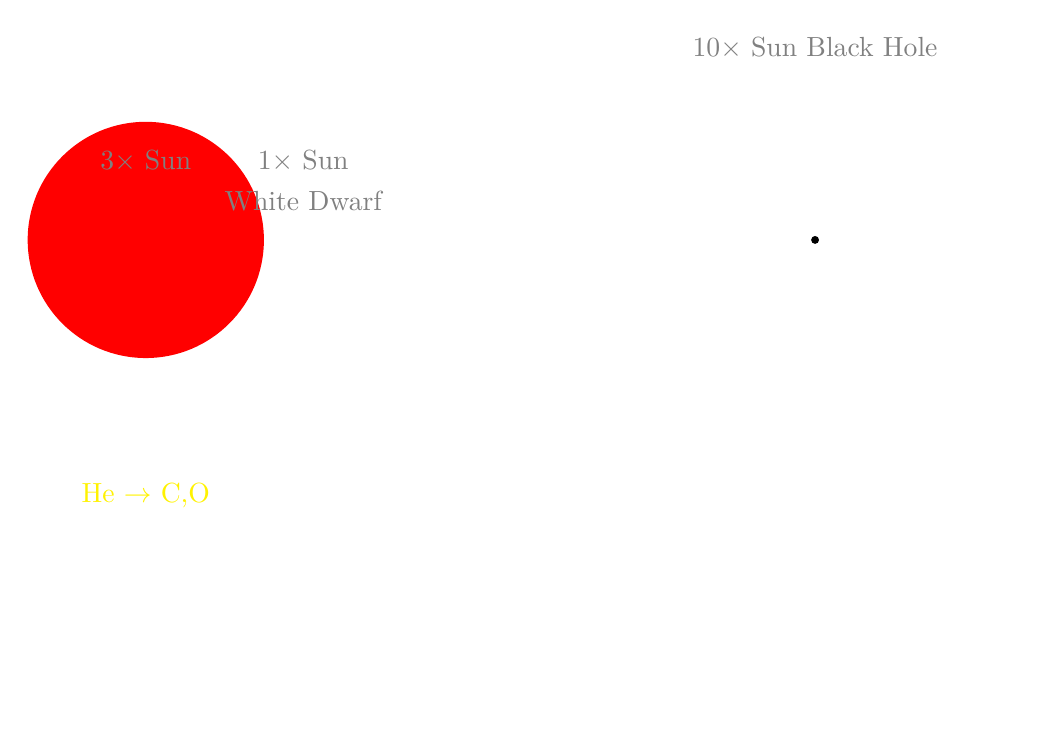
\begin{tikzpicture}
\draw[opacity=0] (0.1,0.1) rectangle (12.6,8.6);


\fill[red] (1.5,6) circle (1.5);
\fill[white] (3.5,6) circle (0.14);
\draw[white!50!black] (1.5,7) node {3$\times$ Sun};
\draw[white!50!black] (3.5,7) node {1$\times$ Sun};
\draw[white!50!black] (3.5,6.5) node {White Dwarf};
\draw[yellow] (1.5,2.75) node {He $\rightarrow$ C,O};

\draw[white!50!black] (10,8.44) node {10$\times$ Sun Black Hole};
\fill[black] (10,6) circle (0.05);

\end{tikzpicture}
}
\frame{\frametitle{Three stars: a story : {\color{red} 2.001 Billion Years Old}}
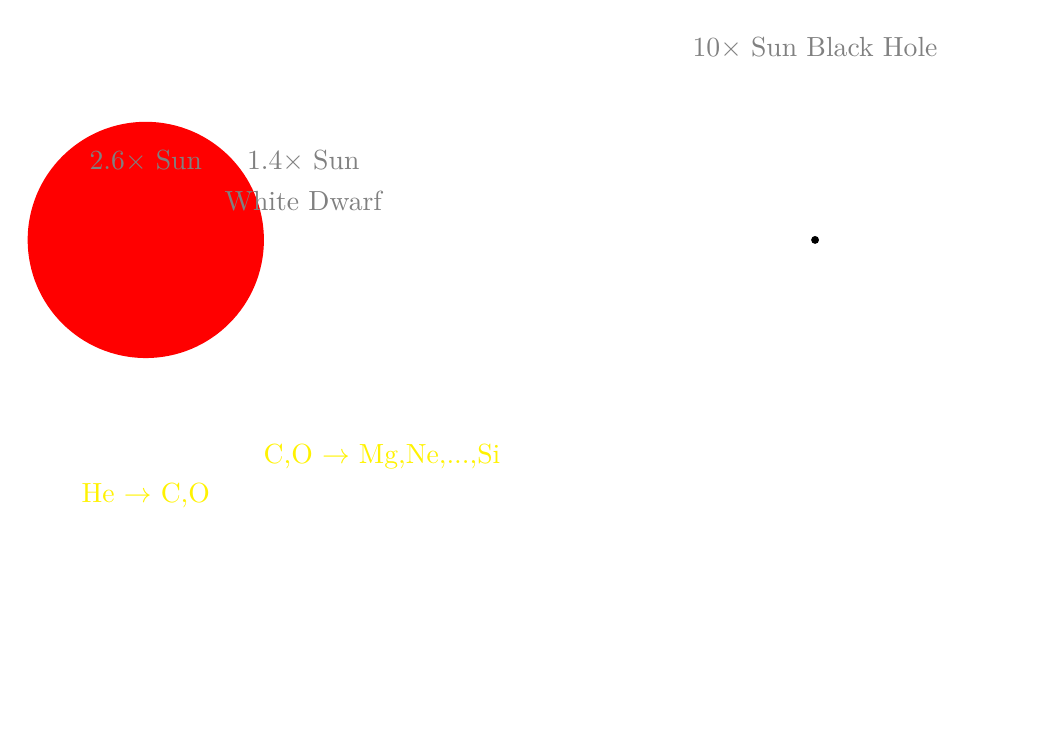
\begin{tikzpicture}
\draw[opacity=0] (0.1,0.1) rectangle (12.6,8.6);


\fill[red] (1.5,6) circle (1.5);
\fill[white] (3.5,6) circle (0.14);
\draw[white!50!black] (1.5,7) node {2.6$\times$ Sun};
\draw[white!50!black] (3.5,7) node {1.4$\times$ Sun};
\draw[white!50!black] (3.5,6.5) node {White Dwarf};
\draw[yellow] (1.5,2.75) node {He $\rightarrow$ C,O};
\draw[yellow] (4.5,3.25) node {C,O $\rightarrow$ Mg,Ne,...,Si};

\draw[white!50!black] (10,8.44) node {10$\times$ Sun Black Hole};
\fill[black] (10,6) circle (0.05);

\end{tikzpicture}
}

\frame{\frametitle{Three stars: a story : {\color{red} 2.001 Billion Years Old + 100 years}}
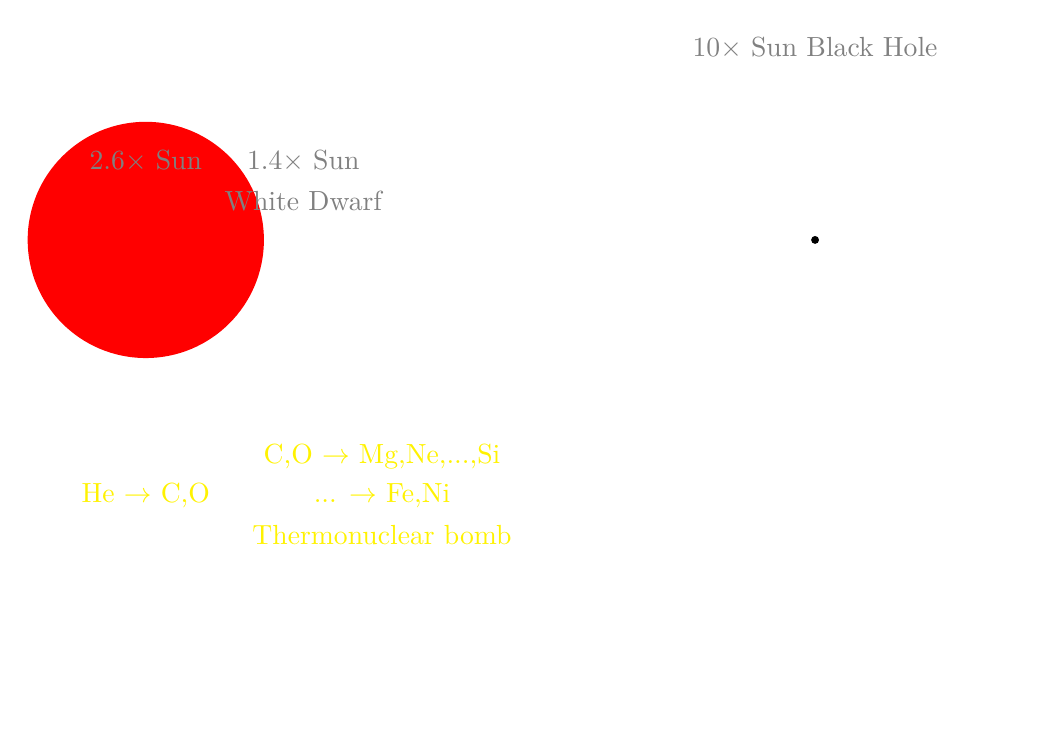
\begin{tikzpicture}
\draw[opacity=0] (0.1,0.1) rectangle (12.6,8.6);


\fill[red] (1.5,6) circle (1.5);
\fill[white] (3.5,6) circle (0.14);
\draw[white!50!black] (1.5,7) node {2.6$\times$ Sun};
\draw[white!50!black] (3.5,7) node {1.4$\times$ Sun};
\draw[white!50!black] (3.5,6.5) node {White Dwarf};
\draw[yellow] (1.5,2.75) node {He $\rightarrow$ C,O};
\draw[yellow] (4.5,3.25) node {C,O $\rightarrow$ Mg,Ne,...,Si};
\draw[yellow] (4.5,2.75) node {... $\rightarrow$ Fe,Ni};
\draw[yellow] (4.5,2.25) node {Thermonuclear bomb};

\draw[white!50!black] (10,8.44) node {10$\times$ Sun Black Hole};
\fill[black] (10,6) circle (0.05);

\end{tikzpicture}
}
\frame{\frametitle{Three stars: a story :\\ {\color{red} 2.001 Billion Years Old + 100 years + 3s}}
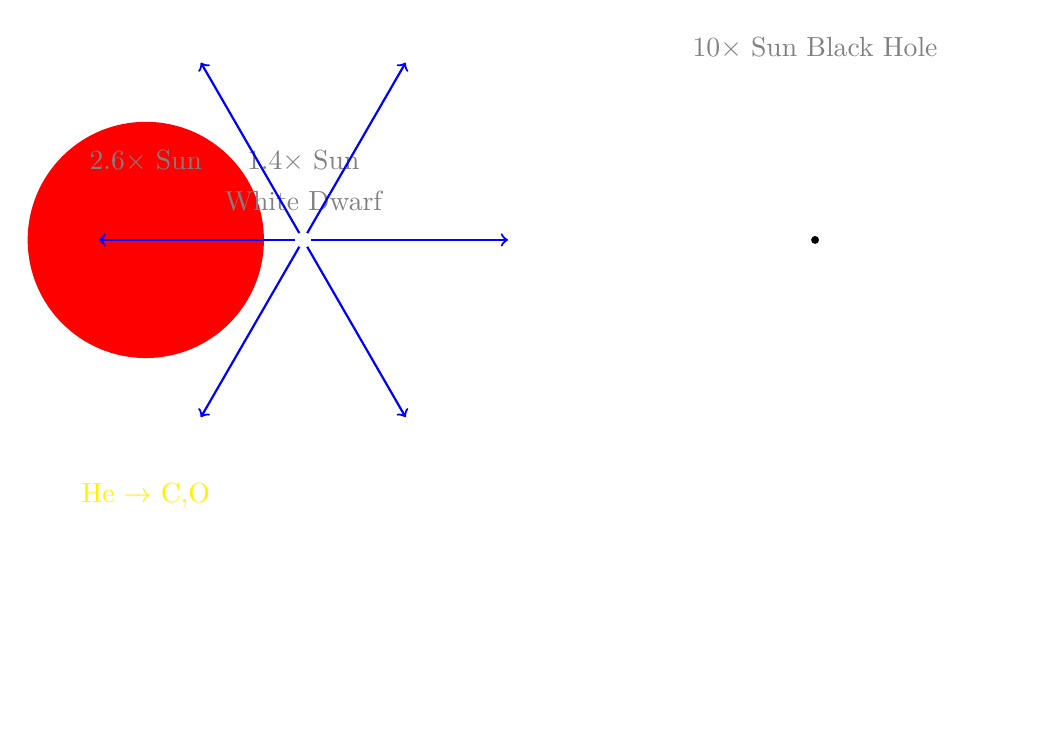
\begin{tikzpicture}
\draw[opacity=0] (0.1,0.1) rectangle (12.6,8.6);


\fill[red] (1.5,6) circle (1.5);
\fill[white] (3.5,6) circle (0.14);
\draw[white!50!black] (1.5,7) node {2.6$\times$ Sun};
\draw[white!50!black] (3.5,7) node {1.4$\times$ Sun};
\draw[white!50!black] (3.5,6.5) node {White Dwarf};
\foreach \x in {0,60,-60,120,-120,180}
{
	\draw[blue,thick,->] (3.5,6)++(\x:0.1) -- +(\x:2.5);
} 
\draw[yellow] (1.5,2.75) node {He $\rightarrow$ C,O};

\draw[white!50!black] (10,8.44) node {10$\times$ Sun Black Hole};
\fill[black] (10,6) circle (0.05);

\end{tikzpicture}
}

\frame{\frametitle{A supernova remnant: Tycho's supernova\\ {\small \color{red} 433 years after the explosion}}
\begin{tikzpicture}
\draw[opacity=0] (0.1,0.1) rectangle (12.6,8.6);

\tkzpic{0.9}{0.2}{11}{8.25}{Pictures/tycho};
\draw[yellow] (2.5,7.95) -- (2.5,8.0) -- (10.3,8.0) -- (10.3,7.95);
\draw[yellow] (6.4,8.25) node {11 light years};
\draw[yellow!50!red] (10.6,5.5) -- (11.0,5.625) node[right] {Hot gas};
\draw[yellow!50!red] (6.2,7.5) -- (11.0,7.625) node[right] {Dust};

\draw[yellow] (6.4,0.85) node[font=\tiny] {Credit: NASA/CXC/Rutgers/J.Warren \& J.Hughes et al.}; 
\end{tikzpicture}
}

\frame{\frametitle{Expansion \& Dark Energy}
\begin{tikzpicture}
\draw[opacity=0] (0.1,0.1) rectangle (15.8,9);
\draw[yellow] (7.9,8.25) node {No Expansion};
\begin{scope}[even odd rule]
\clip (2,7.50) circle (0.45);
\tkzpic{1.5}{7.00}{1}{1}{Pictures/tycho};
\end{scope}
\begin{scope}[even odd rule]
\clip (14.5,7.50) circle (0.25);
\tkzpic{14.25}{7.25}{0.5}{0.5}{Pictures/115334main_image_feature_329_ys_full};
\end{scope}
\draw[white!75!gray,rounded corners] (2.80,7.50) -- (2.90,7.50) -- (3.00,7.80) -- (3.10,7.50) -- (3.20,7.20) -- (3.30,7.50) -- (3.40,7.50);
\draw[yellow] (7.9,6.25) node {Constant Expansion};
\begin{scope}[even odd rule]
\clip (2,5.50) circle (0.45);
\tkzpic{1.5}{5.00}{1}{1}{Pictures/tycho};
\end{scope}
\begin{scope}[even odd rule]
\clip (14.5,5.50) circle (0.25);
\tkzpic{14.25}{5.25}{0.5}{0.5}{Pictures/115334main_image_feature_329_ys_full};
\end{scope}
\draw[white!75!gray,rounded corners] (2.80,5.50) -- (2.90,5.50) -- (3.00,5.80) -- (3.10,5.50) -- (3.20,5.20) -- (3.30,5.50) -- (3.40,5.50);
\draw[yellow] (7.9,4.25) node {Dark Energy};
\begin{scope}[even odd rule]
\clip (2,3.50) circle (0.45);
\tkzpic{1.5}{3.00}{1}{1}{Pictures/tycho};
\end{scope}
\begin{scope}[even odd rule]
\clip (14.5,3.50) circle (0.25);
\tkzpic{14.25}{3.25}{0.5}{0.5}{Pictures/115334main_image_feature_329_ys_full};
\end{scope}
\draw[white!75!gray,rounded corners] (2.80,3.50) -- (2.90,3.50) -- (3.00,3.80) -- (3.10,3.50) -- (3.20,3.20) -- (3.30,3.50) -- (3.40,3.50);
\end{tikzpicture}
}
\frame{\frametitle{Expansion \& Dark Energy}
\begin{tikzpicture}
\draw[opacity=0] (0.1,0.1) rectangle (15.8,9);
\draw[yellow] (7.9,8.25) node {No Expansion};
\begin{scope}[even odd rule]
\clip (2,7.50) circle (0.45);
\tkzpic{1.5}{7.00}{1}{1}{Pictures/tycho};
\end{scope}
\begin{scope}[even odd rule]
\clip (14.5,7.50) circle (0.25);
\tkzpic{14.25}{7.25}{0.5}{0.5}{Pictures/115334main_image_feature_329_ys_full};
\end{scope}
\draw[white!75!gray,rounded corners] (3.80,7.50) -- (3.90,7.50) -- (4.00,7.80) -- (4.10,7.50) -- (4.20,7.20) -- (4.30,7.50) -- (4.40,7.50);
\draw[yellow] (7.9,6.25) node {Constant Expansion};
\begin{scope}[even odd rule]
\clip (2,5.50) circle (0.45);
\tkzpic{1.5}{5.00}{1}{1}{Pictures/tycho};
\end{scope}
\begin{scope}[even odd rule]
\clip (14.5,5.50) circle (0.25);
\tkzpic{14.25}{5.25}{0.5}{0.5}{Pictures/115334main_image_feature_329_ys_full};
\end{scope}
\draw[white!75!gray,rounded corners] (3.74,5.50) -- (3.86,5.50) -- (3.98,5.80) -- (4.10,5.50) -- (4.22,5.20) -- (4.34,5.50) -- (4.46,5.50);
\draw[yellow] (7.9,4.25) node {Dark Energy};
\begin{scope}[even odd rule]
\clip (2,3.50) circle (0.45);
\tkzpic{1.5}{3.00}{1}{1}{Pictures/tycho};
\end{scope}
\begin{scope}[even odd rule]
\clip (14.5,3.50) circle (0.25);
\tkzpic{14.25}{3.25}{0.5}{0.5}{Pictures/115334main_image_feature_329_ys_full};
\end{scope}
\draw[white!75!gray,rounded corners] (3.74,3.50) -- (3.86,3.50) -- (3.98,3.80) -- (4.10,3.50) -- (4.22,3.20) -- (4.34,3.50) -- (4.46,3.50);
\end{tikzpicture}
}
\frame{\frametitle{Expansion \& Dark Energy}
\begin{tikzpicture}
\draw[opacity=0] (0.1,0.1) rectangle (15.8,9);
\draw[yellow] (7.9,8.25) node {No Expansion};
\begin{scope}[even odd rule]
\clip (2,7.50) circle (0.45);
\tkzpic{1.5}{7.00}{1}{1}{Pictures/tycho};
\end{scope}
\begin{scope}[even odd rule]
\clip (14.5,7.50) circle (0.25);
\tkzpic{14.25}{7.25}{0.5}{0.5}{Pictures/115334main_image_feature_329_ys_full};
\end{scope}
\draw[white!75!gray,rounded corners] (4.80,7.50) -- (4.90,7.50) -- (5.00,7.80) -- (5.10,7.50) -- (5.20,7.20) -- (5.30,7.50) -- (5.40,7.50);
\draw[yellow] (7.9,6.25) node {Constant Expansion};
\begin{scope}[even odd rule]
\clip (2,5.50) circle (0.45);
\tkzpic{1.5}{5.00}{1}{1}{Pictures/tycho};
\end{scope}
\begin{scope}[even odd rule]
\clip (14.5,5.50) circle (0.25);
\tkzpic{14.25}{5.25}{0.5}{0.5}{Pictures/115334main_image_feature_329_ys_full};
\end{scope}
\draw[white!75!gray,rounded corners] (4.68,5.50) -- (4.82,5.50) -- (4.96,5.80) -- (5.10,5.50) -- (5.24,5.20) -- (5.38,5.50) -- (5.52,5.50);
\draw[yellow] (7.9,4.25) node {Dark Energy};
\begin{scope}[even odd rule]
\clip (2,3.50) circle (0.45);
\tkzpic{1.5}{3.00}{1}{1}{Pictures/tycho};
\end{scope}
\begin{scope}[even odd rule]
\clip (14.5,3.50) circle (0.25);
\tkzpic{14.25}{3.25}{0.5}{0.5}{Pictures/115334main_image_feature_329_ys_full};
\end{scope}
\draw[white!75!gray,rounded corners] (4.66,3.50) -- (4.81,3.50) -- (4.95,3.80) -- (5.10,3.50) -- (5.25,3.20) -- (5.39,3.50) -- (5.54,3.50);
\end{tikzpicture}
}
\frame{\frametitle{Expansion \& Dark Energy}
\begin{tikzpicture}
\draw[opacity=0] (0.1,0.1) rectangle (15.8,9);
\draw[yellow] (7.9,8.25) node {No Expansion};
\begin{scope}[even odd rule]
\clip (2,7.50) circle (0.45);
\tkzpic{1.5}{7.00}{1}{1}{Pictures/tycho};
\end{scope}
\begin{scope}[even odd rule]
\clip (14.5,7.50) circle (0.25);
\tkzpic{14.25}{7.25}{0.5}{0.5}{Pictures/115334main_image_feature_329_ys_full};
\end{scope}
\draw[white!75!gray,rounded corners] (5.80,7.50) -- (5.90,7.50) -- (6.00,7.80) -- (6.10,7.50) -- (6.20,7.20) -- (6.30,7.50) -- (6.40,7.50);
\draw[yellow] (7.9,6.25) node {Constant Expansion};
\begin{scope}[even odd rule]
\clip (2,5.50) circle (0.45);
\tkzpic{1.5}{5.00}{1}{1}{Pictures/tycho};
\end{scope}
\begin{scope}[even odd rule]
\clip (14.5,5.50) circle (0.25);
\tkzpic{14.25}{5.25}{0.5}{0.5}{Pictures/115334main_image_feature_329_ys_full};
\end{scope}
\draw[white!75!gray,rounded corners] (5.62,5.50) -- (5.78,5.50) -- (5.94,5.80) -- (6.10,5.50) -- (6.26,5.20) -- (6.42,5.50) -- (6.58,5.50);
\draw[yellow] (7.9,4.25) node {Dark Energy};
\begin{scope}[even odd rule]
\clip (2,3.50) circle (0.45);
\tkzpic{1.5}{3.00}{1}{1}{Pictures/tycho};
\end{scope}
\begin{scope}[even odd rule]
\clip (14.5,3.50) circle (0.25);
\tkzpic{14.25}{3.25}{0.5}{0.5}{Pictures/115334main_image_feature_329_ys_full};
\end{scope}
\draw[white!75!gray,rounded corners] (5.58,3.50) -- (5.75,3.50) -- (5.93,3.80) -- (6.10,3.50) -- (6.27,3.20) -- (6.45,3.50) -- (6.62,3.50);
\end{tikzpicture}
}
\frame{\frametitle{Expansion \& Dark Energy}
\begin{tikzpicture}
\draw[opacity=0] (0.1,0.1) rectangle (15.8,9);
\draw[yellow] (7.9,8.25) node {No Expansion};
\begin{scope}[even odd rule]
\clip (2,7.50) circle (0.45);
\tkzpic{1.5}{7.00}{1}{1}{Pictures/tycho};
\end{scope}
\begin{scope}[even odd rule]
\clip (14.5,7.50) circle (0.25);
\tkzpic{14.25}{7.25}{0.5}{0.5}{Pictures/115334main_image_feature_329_ys_full};
\end{scope}
\draw[white!75!gray,rounded corners] (6.80,7.50) -- (6.90,7.50) -- (7.00,7.80) -- (7.10,7.50) -- (7.20,7.20) -- (7.30,7.50) -- (7.40,7.50);
\draw[yellow] (7.9,6.25) node {Constant Expansion};
\begin{scope}[even odd rule]
\clip (2,5.50) circle (0.45);
\tkzpic{1.5}{5.00}{1}{1}{Pictures/tycho};
\end{scope}
\begin{scope}[even odd rule]
\clip (14.5,5.50) circle (0.25);
\tkzpic{14.25}{5.25}{0.5}{0.5}{Pictures/115334main_image_feature_329_ys_full};
\end{scope}
\draw[white!75!gray,rounded corners] (6.56,5.50) -- (6.74,5.50) -- (6.92,5.80) -- (7.10,5.50) -- (7.28,5.20) -- (7.46,5.50) -- (7.64,5.50);
\draw[yellow] (7.9,4.25) node {Dark Energy};
\begin{scope}[even odd rule]
\clip (2,3.50) circle (0.45);
\tkzpic{1.5}{3.00}{1}{1}{Pictures/tycho};
\end{scope}
\begin{scope}[even odd rule]
\clip (14.5,3.50) circle (0.25);
\tkzpic{14.25}{3.25}{0.5}{0.5}{Pictures/115334main_image_feature_329_ys_full};
\end{scope}
\draw[white!75!gray,rounded corners] (6.49,3.50) -- (6.69,3.50) -- (6.90,3.80) -- (7.10,3.50) -- (7.30,3.20) -- (7.51,3.50) -- (7.71,3.50);
\end{tikzpicture}
}
\frame{\frametitle{Expansion \& Dark Energy}
\begin{tikzpicture}
\draw[opacity=0] (0.1,0.1) rectangle (15.8,9);
\draw[yellow] (7.9,8.25) node {No Expansion};
\begin{scope}[even odd rule]
\clip (2,7.50) circle (0.45);
\tkzpic{1.5}{7.00}{1}{1}{Pictures/tycho};
\end{scope}
\begin{scope}[even odd rule]
\clip (14.5,7.50) circle (0.25);
\tkzpic{14.25}{7.25}{0.5}{0.5}{Pictures/115334main_image_feature_329_ys_full};
\end{scope}
\draw[white!75!gray,rounded corners] (7.80,7.50) -- (7.90,7.50) -- (8.00,7.80) -- (8.10,7.50) -- (8.20,7.20) -- (8.30,7.50) -- (8.40,7.50);
\draw[yellow] (7.9,6.25) node {Constant Expansion};
\begin{scope}[even odd rule]
\clip (2,5.50) circle (0.45);
\tkzpic{1.5}{5.00}{1}{1}{Pictures/tycho};
\end{scope}
\begin{scope}[even odd rule]
\clip (14.5,5.50) circle (0.25);
\tkzpic{14.25}{5.25}{0.5}{0.5}{Pictures/115334main_image_feature_329_ys_full};
\end{scope}
\draw[white!75!gray,rounded corners] (7.50,5.50) -- (7.70,5.50) -- (7.90,5.80) -- (8.10,5.50) -- (8.30,5.20) -- (8.50,5.50) -- (8.70,5.50);
\draw[yellow] (7.9,4.25) node {Dark Energy};
\begin{scope}[even odd rule]
\clip (2,3.50) circle (0.45);
\tkzpic{1.5}{3.00}{1}{1}{Pictures/tycho};
\end{scope}
\begin{scope}[even odd rule]
\clip (14.5,3.50) circle (0.25);
\tkzpic{14.25}{3.25}{0.5}{0.5}{Pictures/115334main_image_feature_329_ys_full};
\end{scope}
\draw[white!75!gray,rounded corners] (7.39,3.50) -- (7.62,3.50) -- (7.86,3.80) -- (8.10,3.50) -- (8.34,3.20) -- (8.57,3.50) -- (8.81,3.50);
\end{tikzpicture}
}
\frame{\frametitle{Expansion \& Dark Energy}
\begin{tikzpicture}
\draw[opacity=0] (0.1,0.1) rectangle (15.8,9);
\draw[yellow] (7.9,8.25) node {No Expansion};
\begin{scope}[even odd rule]
\clip (2,7.50) circle (0.45);
\tkzpic{1.5}{7.00}{1}{1}{Pictures/tycho};
\end{scope}
\begin{scope}[even odd rule]
\clip (14.5,7.50) circle (0.25);
\tkzpic{14.25}{7.25}{0.5}{0.5}{Pictures/115334main_image_feature_329_ys_full};
\end{scope}
\draw[white!75!gray,rounded corners] (8.80,7.50) -- (8.90,7.50) -- (9.00,7.80) -- (9.10,7.50) -- (9.20,7.20) -- (9.30,7.50) -- (9.40,7.50);
\draw[yellow] (7.9,6.25) node {Constant Expansion};
\begin{scope}[even odd rule]
\clip (2,5.50) circle (0.45);
\tkzpic{1.5}{5.00}{1}{1}{Pictures/tycho};
\end{scope}
\begin{scope}[even odd rule]
\clip (14.5,5.50) circle (0.25);
\tkzpic{14.25}{5.25}{0.5}{0.5}{Pictures/115334main_image_feature_329_ys_full};
\end{scope}
\draw[white!75!gray,rounded corners] (8.44,5.50) -- (8.66,5.50) -- (8.88,5.80) -- (9.10,5.50) -- (9.32,5.20) -- (9.54,5.50) -- (9.76,5.50);
\draw[yellow] (7.9,4.25) node {Dark Energy};
\begin{scope}[even odd rule]
\clip (2,3.50) circle (0.45);
\tkzpic{1.5}{3.00}{1}{1}{Pictures/tycho};
\end{scope}
\begin{scope}[even odd rule]
\clip (14.5,3.50) circle (0.25);
\tkzpic{14.25}{3.25}{0.5}{0.5}{Pictures/115334main_image_feature_329_ys_full};
\end{scope}
\draw[white!75!gray,rounded corners] (8.28,3.50) -- (8.55,3.50) -- (8.83,3.80) -- (9.10,3.50) -- (9.37,3.20) -- (9.65,3.50) -- (9.92,3.50);
\end{tikzpicture}
}
\frame{\frametitle{Expansion \& Dark Energy}
\begin{tikzpicture}
\draw[opacity=0] (0.1,0.1) rectangle (15.8,9);
\draw[yellow] (7.9,8.25) node {No Expansion};
\begin{scope}[even odd rule]
\clip (2,7.50) circle (0.45);
\tkzpic{1.5}{7.00}{1}{1}{Pictures/tycho};
\end{scope}
\begin{scope}[even odd rule]
\clip (14.5,7.50) circle (0.25);
\tkzpic{14.25}{7.25}{0.5}{0.5}{Pictures/115334main_image_feature_329_ys_full};
\end{scope}
\draw[white!75!gray,rounded corners] (9.80,7.50) -- (9.90,7.50) -- (10.00,7.80) -- (10.10,7.50) -- (10.20,7.20) -- (10.30,7.50) -- (10.40,7.50);
\draw[yellow] (7.9,6.25) node {Constant Expansion};
\begin{scope}[even odd rule]
\clip (2,5.50) circle (0.45);
\tkzpic{1.5}{5.00}{1}{1}{Pictures/tycho};
\end{scope}
\begin{scope}[even odd rule]
\clip (14.5,5.50) circle (0.25);
\tkzpic{14.25}{5.25}{0.5}{0.5}{Pictures/115334main_image_feature_329_ys_full};
\end{scope}
\draw[white!75!gray,rounded corners] (9.38,5.50) -- (9.62,5.50) -- (9.86,5.80) -- (10.10,5.50) -- (10.34,5.20) -- (10.58,5.50) -- (10.82,5.50);
\draw[yellow] (7.9,4.25) node {Dark Energy};
\begin{scope}[even odd rule]
\clip (2,3.50) circle (0.45);
\tkzpic{1.5}{3.00}{1}{1}{Pictures/tycho};
\end{scope}
\begin{scope}[even odd rule]
\clip (14.5,3.50) circle (0.25);
\tkzpic{14.25}{3.25}{0.5}{0.5}{Pictures/115334main_image_feature_329_ys_full};
\end{scope}
\draw[white!75!gray,rounded corners] (9.16,3.50) -- (9.47,3.50) -- (9.79,3.80) -- (10.10,3.50) -- (10.41,3.20) -- (10.73,3.50) -- (11.04,3.50);
\end{tikzpicture}
}
\frame{\frametitle{Expansion \& Dark Energy}
\begin{tikzpicture}
\draw[opacity=0] (0.1,0.1) rectangle (15.8,9);
\draw[yellow] (7.9,8.25) node {No Expansion};
\begin{scope}[even odd rule]
\clip (2,7.50) circle (0.45);
\tkzpic{1.5}{7.00}{1}{1}{Pictures/tycho};
\end{scope}
\begin{scope}[even odd rule]
\clip (14.5,7.50) circle (0.25);
\tkzpic{14.25}{7.25}{0.5}{0.5}{Pictures/115334main_image_feature_329_ys_full};
\end{scope}
\draw[white!75!gray,rounded corners] (10.80,7.50) -- (10.90,7.50) -- (11.00,7.80) -- (11.10,7.50) -- (11.20,7.20) -- (11.30,7.50) -- (11.40,7.50);
\draw[yellow] (7.9,6.25) node {Constant Expansion};
\begin{scope}[even odd rule]
\clip (2,5.50) circle (0.45);
\tkzpic{1.5}{5.00}{1}{1}{Pictures/tycho};
\end{scope}
\begin{scope}[even odd rule]
\clip (14.5,5.50) circle (0.25);
\tkzpic{14.25}{5.25}{0.5}{0.5}{Pictures/115334main_image_feature_329_ys_full};
\end{scope}
\draw[white!75!gray,rounded corners] (10.32,5.50) -- (10.58,5.50) -- (10.84,5.80) -- (11.10,5.50) -- (11.36,5.20) -- (11.62,5.50) -- (11.88,5.50);
\draw[yellow] (7.9,4.25) node {Dark Energy};
\begin{scope}[even odd rule]
\clip (2,3.50) circle (0.45);
\tkzpic{1.5}{3.00}{1}{1}{Pictures/tycho};
\end{scope}
\begin{scope}[even odd rule]
\clip (14.5,3.50) circle (0.25);
\tkzpic{14.25}{3.25}{0.5}{0.5}{Pictures/115334main_image_feature_329_ys_full};
\end{scope}
\draw[white!75!gray,rounded corners] (10.03,3.50) -- (10.39,3.50) -- (10.74,3.80) -- (11.10,3.50) -- (11.46,3.20) -- (11.81,3.50) -- (12.17,3.50);
\end{tikzpicture}
}
\frame{\frametitle{Expansion \& Dark Energy}
\begin{tikzpicture}
\draw[opacity=0] (0.1,0.1) rectangle (15.8,9);
\draw[yellow] (7.9,8.25) node {No Expansion};
\begin{scope}[even odd rule]
\clip (2,7.50) circle (0.45);
\tkzpic{1.5}{7.00}{1}{1}{Pictures/tycho};
\end{scope}
\begin{scope}[even odd rule]
\clip (14.5,7.50) circle (0.25);
\tkzpic{14.25}{7.25}{0.5}{0.5}{Pictures/115334main_image_feature_329_ys_full};
\end{scope}
\draw[white!75!gray,rounded corners] (11.80,7.50) -- (11.90,7.50) -- (12.00,7.80) -- (12.10,7.50) -- (12.20,7.20) -- (12.30,7.50) -- (12.40,7.50);
\draw[yellow] (7.9,6.25) node {Constant Expansion};
\begin{scope}[even odd rule]
\clip (2,5.50) circle (0.45);
\tkzpic{1.5}{5.00}{1}{1}{Pictures/tycho};
\end{scope}
\begin{scope}[even odd rule]
\clip (14.5,5.50) circle (0.25);
\tkzpic{14.25}{5.25}{0.5}{0.5}{Pictures/115334main_image_feature_329_ys_full};
\end{scope}
\draw[white!75!gray,rounded corners] (11.26,5.50) -- (11.54,5.50) -- (11.82,5.80) -- (12.10,5.50) -- (12.38,5.20) -- (12.66,5.50) -- (12.94,5.50);
\draw[yellow] (7.9,4.25) node {Dark Energy};
\begin{scope}[even odd rule]
\clip (2,3.50) circle (0.45);
\tkzpic{1.5}{3.00}{1}{1}{Pictures/tycho};
\end{scope}
\begin{scope}[even odd rule]
\clip (14.5,3.50) circle (0.25);
\tkzpic{14.25}{3.25}{0.5}{0.5}{Pictures/115334main_image_feature_329_ys_full};
\end{scope}
\draw[white!75!gray,rounded corners] (10.90,3.50) -- (11.30,3.50) -- (11.70,3.80) -- (12.10,3.50) -- (12.50,3.20) -- (12.90,3.50) -- (13.30,3.50);
\end{tikzpicture}
}

%\frame{
%\frametitle{What they aren't}
%\begin{tikzpicture}
%\draw[opacity=0] (0.1,0.1) rectangle (12.6,8.6);

%\fill[yellow] (7.85,2) circle(7);
%\draw[black] (7.85,6) node {A Sun-like (1 -- $\sim 8\;\mathrm{M}_\odot$) star};
%\draw[red] (7.85,3) node {Too much hydrogen};
%\foreach \x in {0,30,-30,150,-150,180}
%{%
%	\draw[red,thick,->] (7.85,3)++(\x:2) -- +(\x:4);
%} 
%\draw[white]  (7.85,2) circle(0.07);
%\end{tikzpicture}
%}

%\frame{
%\frametitle{But, strip away the hydrogen}
%\begin{tikzpicture}
%\draw[opacity=0] (0.1,0.1) rectangle (12.6,8.6);

%\fill[white]  (7.85,2) circle(0.07);
%\draw[white] (7.85,2.5) node {White dwarf};
%\draw[white] (7.85,1.5) node {Former core of sun-like star};
%\draw[white] (7.85,1.0) node {About the size of Earth};

%\end{tikzpicture}
%}

\frame{\frametitle{Summary}
\begin{centering}
\vspace{0.5cm}
Supernova = Exploding star\hfill\\[14pt]
Factories for {\color{gray}neutron stars} \& {\color{black}\bf black holes}\\
{\scriptsize Only source of {\color{gray}neutron stars}}\\
{\scriptsize Maybe only source of {\color{black}\bf black holes}}\\[14pt]
Source of most elements${}^*$ heaver than oxygen in the Universe\\
{\scriptsize All of the {\color{red}iron} in your blood and {\color{yellow}calcium} in your bones were formed in supernovae}\\
{\scriptsize ${}^*$ elements heavier than {\color{green}copper} also come from {\color{gray}neutron star} mergers}\\
{\scriptsize ${}^*$ some elements heavier than {\color{magenta}strontium} also come from red giants}\\[14pt]
Thermonuclear supernovae reveal the presence of \color{magenta}{dark energy}.\\


\end{centering}
}

\section*{bibliography}


\end{document}

